\PassOptionsToPackage{final}{graphicx}
\PassOptionsToPackage{final}{listings}
\documentclass{llncs}
\usepackage[utf8]{inputenc}
\usepackage[vlined,linesnumbered]{algorithm2e}
\usepackage{amsopn}
\usepackage{amsmath}
\usepackage{amsfonts}
\usepackage{thmtools,thm-restate}
\usepackage{bm}
\usepackage{caption} 
\usepackage{sansmath}
\usepackage{amssymb}
%\usepackage[francais]{babel}
%\usepackage[utf8]{inputenc}
\usepackage{amsmath}
\usepackage{amssymb}
\usepackage{amsfonts}
\usepackage{amsopn}
\usepackage{amscd}
\usepackage[bookmarks=false]{hyperref}
\usepackage{verbatim}
\usepackage{subfig}
\usepackage{tikz}
\usepackage{proof}
\usepackage{alltt}
\usepackage{color}
\usepackage{xspace}
% \usepackage{ifthen}
% \usepackage{fancybox}
\usepackage{wrapfig}
% \usepackage{multirow}
% \usepackage{listings}
\usepackage{rotating}
\usepackage{xcolor,colortbl}
%\usepackage[textsize=small,colorinlistoftodos]{todonotes}
\usepackage[outdir=./]{epstopdf}
\usepackage{sansmath}
% \usepackage{uppaal}
% \usepackage{longtable}
\usepackage[square,numbers,sectionbib]{natbib}

%% to highlight changes using \added{...}, \deleted{...}, \replaced{...}{...}
%\usepackage{changes}
\usepackage[inline]{enumitem}

%%% Local Variables:
%%% mode: latex
%%% TeX-master: "main"
%%% End:

% \newcommand{\delay}{\ensuremath{\mathbb{Delay}}\xspace}

\newcommand{\parfunc}{\hookrightarrow}
\newcommand{\changethis}[1]{{\em {\color{red} #1}\/}}
\newcommand{\mean}{\mathtt{M}}
\newcommand{\variance}{\mathtt{V}}
\newcommand{\welche}{\mathtt{W}}
\newcommand{\kstest}{\mathtt{KS}}
\newcommand{\refinetest}{\mathtt{DIF}}
\newcommand{\cp}{\mathtt{LMS}}
\newcommand{\cpcnt}{\mathtt{LMSVal}}
\newcommand{\lowdif}{\triangleleft}
\newcommand{\highdif}{\triangleright}
\newcommand{\middif}{\nmid}
\newcommand{\indif}{\bullet}
\newcommand{\either}{\bowtie}
\newcommand{\statsplus}{\oplus}
\newcommand{\statsmult}{\otimes}

\newcommand{\powerk}{2^{\reals^K}}
\newcommand{\refine}{\rho}
\newcommand{\Refine}{\mathtt{R}}
\newcommand{\splitprob}{\overline{\mathtt{p}}}
\newcommand{\NDist}{\Xi}
\newcommand{\ndist}{\xi}
\newcommand{\stats}{\mathtt{Stats}}

\newcommand{\dee}{\mathrm{d}}


\newcommand{\partition}{\mathcal{A}}
\newcommand{\partitionB}{\mathcal{B}}
\newcommand{\allpart}{\mathbb{A}}

\newcommand{\cylinder}{\ensuremath{\zeta}}

\newcommand{\nnul}{\mathbb{N}_0}

\newcommand{\delay}{\ensuremath{\text{delay}}\xspace}

\newcommand{\trans}[1]{\stackrel{#1}{\longrightarrow}}

\newcommand{\states}{\mathcal{S}}
\newcommand{\initial}{s_{init}}
\newcommand{\reals}{\mathbb{R}}
\newcommand{\rationals}{\mathbb{Q}}
\newcommand{\naturals}{\mathbb{N}}
\newcommand{\mdp}{\mathcal{M}}
\newcommand{\clocks}{\mathcal{X}}
\newcommand{\locs}{\mathcal{L}}
\newcommand{\dist}{\Delta}
\newcommand{\borel}{\mathcal{B}}
\newcommand{\borelk}{{\borel(\reals)^K}}
\newcommand{\run}{\pi}
\newcommand{\runs}{\Pi}
\renewcommand{\path}{\bar{\pi}}
\newcommand{\transitions}{T}
\newcommand{\density}{\Delta}

\newcommand{\act}{\mathit{Act}}
\newcommand{\est}{\mathcal{E}}
\newcommand{\eest}{\hat{\est}}
\newcommand{\pr}{\mathbb{P}}
\newcommand{\epr}{\hat{\pr}}
\newcommand{\freq}{\mathcal{F}}
\newcommand{\efreq}{\hat{\freq}}
\newcommand{\reward}{{\color{red} \mathcal{R} \text{ (SHOULD BE COST!)}}}
\newcommand{\cost}{\mathcal{C}}
\newcommand{\ecost}{\hat{\cost}}
\newcommand{\bb}{\mathit{BB}}
\newcommand{\BB}{\mathbb{B}}
\newcommand{\eerror}{\mathit{EE}}
\newcommand{\tree}{\mathcal{T}}

\newcommand{\goal}{\mathcal{G}}
\newcommand{\apr}[1]{#1_{\sim}}

\newcommand{\cent}{\odot}


\newcommand{\ft}[1]{{\small\textsf{#1}}}

\newcommand{\opmod}{\textsc{OpenModelica}\xspace}

\def\checkmark{\tikz\fill[scale=0.4](0,.35) -- (.25,0) -- (1,.7) -- (.25,.15) -- cycle;}


\newcommand{\actions}[1]{\ensuremath{\mathtt{A}_{#1}}}
\newcommand{\attActions}{\ensuremath{\actions{a}}}
\newcommand{\defActions}{\ensuremath{\actions{d}}}
\newcommand{\attAct}{\ensuremath{p_a}}
\newcommand{\defAct}{\ensuremath{p_d}}
\newcommand{\lang}[2]{\ensuremath{\mathcal{L}(#1,#2)}}
\newcommand{\langw}[2]{\ensuremath{\mathcal{L}^w(#1,#2)}}
\newcommand{\R}{\ensuremath{\mathbb{R_{\geq 0}}}}
\newcommand{\xdashrightarrow}[1]{\ensuremath{\overset{#1}{\dashrightarrow}}}
\newcommand{\attProf}{\ensuremath{\mu_{A}}}
\newcommand{\subf}{\ensuremath{\mathtt{Sub}}}
\newcommand{\prob}{\ensuremath{F}}
\newcommand{\probability}{\ensuremath{\mathbb{P}}}
\newcommand{\failueprob}{\ensuremath{\mathtt{Fail}}}
\newcommand{\denot}[1]{\ensuremath{\llbracket #1 \rrbracket}}
\newcommand{\true}{\ensuremath{\mathtt{tt}}}
\newcommand{\false}{\ensuremath{\mathtt{ff}}}
\newcommand{\aGraph}[1]{\ensuremath{\mathcal{G}^{#1}}}
\newcommand{\attSelect}{\ensuremath{\gamma_\attacker}}
\newcommand{\defSelect}{\ensuremath{\gamma_\defender}}
\newcommand{\attPosDelay}{\ensuremath{\Delta}}
\newcommand{\attDelay}{\ensuremath{\delta}}
\newcommand{\attSucc}{\ensuremath{{\mathtt{Env}}}}
\newcommand{\attFail}{\ensuremath{\delta_{f}}}

\newcommand{\astates}{\ensuremath{\mathsf{S}}}
\newcommand{\astate}[1][]{\ensuremath{{\mathsf{s}^{#1}}}}
\newcommand{\initastate}[1][]{\ensuremath{{\astate[#1]_{0}}}}
\newcommand{\finalvertices}{\ensuremath{F}}

\newcommand{\vvertices}{\ensuremath{\mathcal{V}^t}}
 \newcommand{\vvertex}[1][]{\ensuremath{{v^t_{#1}}}}
 \newcommand{\initvvertex}[1][]{\ensuremath{\vvertex[#1]^0}}
\newcommand{\vertices}{\ensuremath{\mathcal{V}}}

\newcommand{\vertex}[1][]{\ensuremath{{v_{#1}}}}
 \newcommand{\initvertex}[1][]{\ensuremath{\vertex[#1]^0}}
\newcommand{\initavertex}[1][]{\ensuremath{\vertex[#1]^{\attacker}}}
\newcommand{\adgvtoastates}{\ensuremath{M}}
\newcommand{\selectAttActions}{\ensuremath{Ac}}
\newcommand{\sdefender}{\ensuremath{\defender^\mathcal{S}}}
\newcommand{\sattacker}{\ensuremath{\mathcal{\attacker^S}}}
\newcommand{\tattacker}{\ensuremath{\mathcal{\attacker^\tau}}}
\newcommand{\environment}{\ensuremath{Env}}

\newcommand{\dm}[1]{\ensuremath{\mathop{}\!\mathrm{d} #1}}

\newcommand{\truns}{\ensuremath{\Omega^\tau}}
\newcommand{\dotrans}[2]{\ensuremath{[#1]^{#2}}}
\newcommand{\costW}{\ensuremath{\mathtt{CW}}}
\newcommand{\satis}{\ensuremath{\vDash}}
\newcommand{\nsatis}{\ensuremath{\not\vDash}}

\newcommand{\expected}{\ensuremath{\mathbb{E}}}
\newcommand{\lowbounds}[1]{\ensuremath{\mathcal{B}^\geq(#1)}}
\newcommand{\upbounds}[1]{\ensuremath{\mathcal{B}^\leq(#1)}}
\newcommand{\initloc}[1][]{\ensuremath{\ell^{#1}_0}}
\newcommand{\loc}{\ensuremath{\ell}}
\newcommand{\clock}{\ensuremath{c}}
\newcommand{\taactions}[1][]{\ensuremath{\Sigma_{#1}}}
\newcommand{\oactions}{\ensuremath{\Sigma_o}
}\newcommand{\iactions}{\ensuremath{\Sigma_i}}

\newcommand{\cedges}{\ensuremath{\rightarrow_{C}}}
\newcommand{\uedges}{\ensuremath{\rightarrow_{U}}}
\newcommand{\adtree}[1][]{\ensuremath{\psi_{#1}}}

\DeclareMathOperator*{\argmin}{arg\,min}
\DeclareMathOperator*{\argmax}{arg\,max}
\newcommand{\vals}[1]{\mathcal{V}(#1)}
\newcommand{\valzero}{\val_0}
\newcommand{\oaction}[1]{\ensuremath{#1!}}
\newcommand{\iaction}[1]{\ensuremath{a?}}
\newcommand{\ltsover}[1][\adtree]{\ensuremath{\mathtt{LTS}(#1)}}
\newcommand{\graphover}[1][\adtree]{\ensuremath{\mathtt{Graph}(\adtree)}}
\newcommand{\intervals}{\ensuremath{\mathcal{B(\mathbb{R})}}}

\newcommand{\budget}{\ensuremath{B}}

\newcommand{\cstates}{\ensuremath{\mathcal{C}}}
\newcommand{\cstate}{\ensuremath{c}}

% TA
\DeclareMathAlphabet{\mathpzc}{OT1}{pzc}{m}{it}
\def\A{\ensuremath{\mathcal{A}}\xspace}
\def\N{\ensuremath{\mathcal{N}}\xspace}
\newcommand\vclocks[1][]{\ensuremath{{\mathcal{X}^{\mathtt{V}}_{#1}}}\xspace}
\newcommand\tclocks[1][]{\ensuremath{{\mathcal{X}^{\mathtt{T}}_{#1}}}\xspace}
\newcommand\invars[1][]{\ensuremath{I_{#1}}\xspace}
\newcommand\posreals[0]{\ensuremath{\mathbb{R}_{\geq 0}}\xspace}
\newcommand\guards[0]{\ensuremath{\mathcal{G}}\xspace}
\newcommand\reachable[0]{\ensuremath{\mathcal{R}}\xspace}
\newcommand\val[0]{\ensuremath{\nu}\xspace}
\newcommand\timed[0]{\ensuremath{\mathit{Time}}\xspace}
\newcommand\zones[0]{\ensuremath{\mathcal{Z}}\xspace}
\newcommand\updt[0]{\ensuremath{\mathcal{U}}\xspace}
% arrows
\newcommand{\overarrowi}[1]{\overset{#1}{\rightarrow}}
\newcommand{\overarrow}[1]{
  \mathchoice{\raisebox{-2pt}{ $\overarrowi{#1}$ }}
             {\raisebox{-2pt}{ $\overarrowi{#1}$ }}
             {\raisebox{-2pt}{ $\overarrowi{#1}$ }}
             {\raisebox{-2pt}{ $\overarrowi{#1}$ }}}
             
\newcommand{\longoverarrowi}[1]{\overset{#1}{\longrightarrow}}
\newcommand{\longoverarrow}[1]{
  \mathchoice{\raisebox{-3pt}{ $\longoverarrowi{#1}$ }}
             {\raisebox{-3pt}{ $\longoverarrowi{#1}$ }}
             {\raisebox{-3pt}{ $\longoverarrowi{#1}$ }}
             {\raisebox{-3pt}{ $\longoverarrowi{#1}$ }}}


\newcommand{\clockrates}{\ensuremath{\mathcal{R}}}
\newcommand{\pdf}{\ensuremath{\delta}}
\newcommand{\pmf}{\ensuremath{\gamma}}


\newcommand{\sattackers}{\ensuremath{\mathcal{S}}}

\newcommand{\edges}{\ensuremath{\mathtt{E}}}
\newcommand{\dedges}{\ensuremath{\mathtt{E}_d}}
\newcommand{\reach}{\ensuremath{\mathtt{Reach}}}
\newcommand{\uppaal}{\textsc{Uppaal}\xspace}
\newcommand{\uppaalstratego}{\uppaal \textsc{Stratego}\xspace}
\newcommand{\stratego}{\textsc{Stratego}\xspace}

\newcommand{\pruns}[1]{\ensuremath{P_{#1}}}
\newcommand{\costinfty}{\cost^{\infty}}

\newcommand{\viop}{ \ensuremath{{\cal L}}}
\DeclareMathOperator*{\opt}{opt}
\newcommand{\minmax}{ \ensuremath{\opt}}
\newcommand{\closure}{ \mathit{cl}  }

\newcommand{\cmax}{c_{\emph{max}}}
\newcommand{\costlambda}{\cost_{\lambda}}


\newcommand{\dtv}{d_{\emph{tv}}}
\newcommand{\PNtau}[2]{P^{#1}_{\tau,\alpha^{#2}}}
\newcommand{\ENtau}[2]{\expected ^{#1}_{\tau,\alpha^{#2}}}
\newcommand{\alphamin}{\alpha^{\emph{min}}}
\newcommand{\alphamax}{\alpha^{\emph{max}}}
\newcommand{\alphamean}{\alpha^{\emph{mean}}}
\newcommand{\alphaimin}{\alpha^{\emph{i-min}}}
\newcommand{\alphaimax}{\alpha^{\emph{i-max}}}
\newcommand{\alpharho}{\alpha^{\rho}}

  
\newcommand{\boldsigma}{\boldsymbol{\sigma}}
\pagestyle{plain}

\newcommand{\todo}[1]{\textcolor{blue} {\bf TODO:} \parbox[t]{0.8\textwidth}{#1}}

\title{Reinforcement learning for discretized Euclidean MDPs}

\author{Asger Horn Brorholt
\and Manfred Jaeger
\and Peter Gj{\o}l Jensen
\and Kim Guldstrand Larsen
}

\institute{Department of Computer Science, Aalborg University, Denmark }

\begin{document}
\maketitle

\begin{abstract}
  Modern model checking tools like UPPAAL Stratego provide a rich framework for
modeling cyber-physical systems involving time and continuous state descriptors. A key
objective is to design controllers for such systems that optimize a given objective, e.g.,
minimizing energy consumption. At an abstract level, the controller design problem can be
cast as optimizing a strategy in a continuous (Euclidean) Markov decision process.
Discretization of the continuous state space is a simple yet effective strategy to solve
this optimization problem in a flexible, non-parametric manner. In previous work we have
introduced a reinforcement learning strategy on dynamically refined discretizations, and
we have analyzed at the semantic level approximations of Euclidean MDPs by Imprecise
MDPs. In this paper we are moving to close the gap between the theoretical analysis and the
practical reinforcement learning approach. We introduce several alternative simulation strategies
that on the one hand maintain approximation guarantees as the granularity of the discretization
increases, and on the other hand turns our learning scenario into a standard Q-learning
procedure. The known convergence guarantees for Q-learning then provide theoretical guarantees
for the near-optimality of the strategies we learn for our cyber-physical system models.
\end{abstract}



\section{Introduction}


Modern model-checkers (e.g. PRISM \cite{Prism}, STORM \cite{Storm,COOLMC}, MODEST \cite{Modest}, KeYmaeraX \cite{ KeYmaera}, UPPAAL Stratego \cite{UPPAAL,TACAS15}) are increasingly having a focus on integration of state-of-the-art reinforcement learning (RL) and model checking (MC) \cite{Kim2}.  In this effort RL is leveraged to efficiently construct near-optimal control strategies while model checking techniques are used to give absolute \cite{ATVA14}, probabilistic \cite{Kim1, Kim3} or statistical guarantees \cite{FORTE20} of crucial safety properties.

Most importantly, the existing model checkers offer a variety of rich and mature modelling formalisms for defining Markov decision processes (MDPs) that may be used to run simulations for the off-line training of RL policies. Compared to traditional RL scenarios this allows for a number of  additional capabilities, e.g. in terms of “targeted sampling” of initial states, rare configurations, etc.   The modelling formalisms range from finite state MDPs (STORM, PRISM) to continuous-space (Euclidean) Markov decision processes (EMDPs)  (MODEST, UPPAAL Stratego) and Simulink (KeYmaeraX).  For continuous-space models  abstractions are often used in order to obtain the required guarantees \cite{ HerberAL21, ATVA14}.

Most of the above integrations of RL and model checking rely on external components for the RL training (e.g. Open Gym \cite{COOLMC} and Simulinks RL Toolbox \cite{HerberAL21}).  In contrast the tool UPPAAL Stratego offers its own RL method for continuous-space MDPs \cite{ATVA19}.  Here the learning method is based on a dynamic partition-refinement approach for function approximations providing high flexibility regarding the types of functions that can be approximated, but also closely aligns with continuous-time model-checking techniques, so-called zones. 

The RL method of UPPAAL Stratego has already been applied for the construction of near-optimal controllers in a number of industrial applications including traffic-lights \cite{TRP48}, water management \cite{ADHS21,ATVA22}, floor heating systems \cite{TACAS16}, heat-pumps \cite{TASE22}, as well as distributed fleets of autonomous mobile robots \cite{ICAPS22}.

However, the proven practical usefulness of the system is not fully complemented by theoretical guarantees.
The RL approach in UPPAAL Stratego is based on sampled runs in the continuous state space. This, and the
interleaving with partition-refinement steps, means that classic convergence guarantees for
RL~\cite{jaakkola1993convergence}
in finite state spaces are not directly applicable to this approach. 
In \cite{jaeger2020approximating} we have started to develop theoretical underpinnings of the UPPAAL Stratego
approach by using imprecise Markov decision processe (IMDPs) to  formalize 
partition-based abstractions, and
to approximate EMDPs by standard finite state MDPs that provide upper and lower bounds on the
cost function of the EMDP. This analysis was at the purely semantic level and did not make an explicit
link to the convergence of RL. 

This paper is a step towards closing the gap between the theoretical guarantees of \cite{jaeger2020approximating},
and the algorithmic solutions implemented in UPPAAL Stratego. Our main objective here is to reduce the
RL process in UPPAAL Stratego to standard finite state RL, so that all existing implementations and
convergence guarantees for RL become applicable. This reduction relies on two main components: first,
deviating from \cite{jaeger2020approximating}, we will consider a discounted cost criterion as our objective.
As we will show by a counter-example, a conjecture stated in \cite{jaeger2020approximating} regarding the
asymptotic tightness of upper and lower bounds does not actually hold in the un-discounted case. Second, we
introduce new simulation approaches, such that system runs obtained from these simulations are equivalent
to simulations from a standard finite state MDP. 



\subsection*{Related Work}


We refer to  \cite{ATVA19} and \cite{jaeger2020approximating} for a broader discussion of related
approaches towards abstractions of continuous state space systems. Recent work that is
most closely related to ours are \cite{song2019efficient} and \cite{sinclair2019adaptive} which
also develop RL in continuous spaces via finite state space partitionings (or, more generally,
finite \emph{coverings} of the state space). Whereas \cite{song2019efficient} works with a fixed partitioning,
\cite{sinclair2019adaptive} develops an approach for adaptive refinement of the partitions during learning.
In contrast to our work, the authors here assume that the
real systems can not be simulated, and hence can not be used for generating data for offline learning.
As a result, the focus is on minimizing \emph{regret}, i.e., the difference between the
expected   rewards received during training, and the expected rewards under an optimal policy. The analysis
is performed for processes with a fixed time horizon, and the criterion of total (non-discounted) rewards
accumulated up to that time horizon. This differs from our focus on infinite horizon processes with
discounted costs, and the
ability to exploit system models for flexible and efficient data generation. 


\section{Euclidean MDPs}

We start by introducing our continuous state space system model. The definitions in this and the
following section mostly follow \cite{jaeger2020approximating}, but with a few simplifications
that only incur a loss of non-essential generality.

\begin{definition}[Euclidean Markov Decision Processes]\label{def:mdp}
  A      Euclidean Markov decision process        (EMDP)
  is              a              tuple
  $\mdp=(\states, \act, \transitions, \cost)$ where:
\begin{itemize}
\item $\states \subseteq  \reals^K$ is a
 compact subset of the $K$-dimensional Euclidean space equipped with the Borel $\sigma$-algebra
  $\borel^K$. 
\item $\act$ is a finite set of actions,
%\item $\initial\in\states$ is the initial state,
\item    $T:\states    \times   \act  \times\borel^K \rightarrow[0,1]$ defines for every $a\in\act$ a
  transition kernel on $(\states,\borel^K)$,
  i.e., $T(s,a,\cdot)$ is a probability distribution on $\borel^K$ for all
  $s\in\states$, and $T(\cdot,a,B)$ is measurable for all $B\in\borel^K$.
\item  $\cost:\states\times\act\rightarrow[0,\cmax]$   is  a
  cost-function for state-action pairs, such that for all $a\in\act$:
  $\cost(\cdot,a)$ is measurable, and $\cmax$ is a global upper bound on costs.
\end{itemize}
\end{definition}


\begin{figure}
\centering
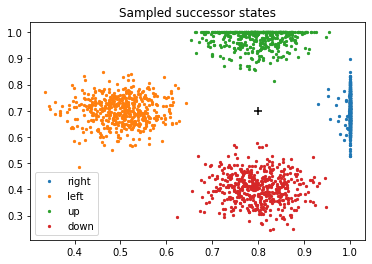
\includegraphics[scale=0.4]{./Figures/successorstates.png}\hspace{5mm}
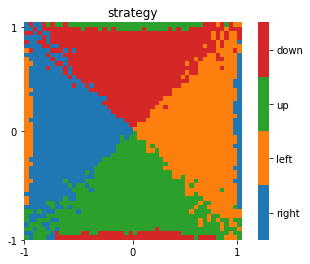
\includegraphics[scale=0.4]{./Figures/strategy.png}
\caption{Sampled successor states and strategy in Example~\ref{ex:2dex} and Example~\ref{ex:2dex-2}
\label{fig:succstates}}
\end{figure}
\begin{example}
\label{ex:2dex}
The following toy example describes a moving agent in a square in the 2d-plane.
Let $\states=[-1,1]\times [-1,1]$, $\act=\{\emph{right},\emph{left},\emph{up},\emph{down}\}$. For
$(x,y)\in \states$, let $T((x,y),\emph{right},\cdot)$ be
$\emph{clip}((x,y)+(0.3,0)+N({\boldsymbol 0},0.003))$, where $N({\boldsymbol 0},0.003))$ is a Gaussian noise
vector with zero mean and diagonal covariance matrix with values 0.003, and
$\emph{clip}(x):=\max\{-1,\min\{1,x\}\}$  ensures that the result stays in $\states$.
The transition probabilities given the other three actions are defined analogously.
Figure~\ref{fig:succstates} on the left shows for the state $s=(0.8,0.7)$ (marked by a black $+$)
samples of 500 successor states according
to $T(s,a,\cdot)$ for each $a\in\act$.
The cost function 
\begin{equation}
\label{eq:2dcosts}
\cost((x,y),\emph{right})= 2*(x^2+y^2)+0.6(1-x)
\end{equation}
consists of two elements: a cost proportional to the squared Euclidean distance to the origin, and a cost
that is inversely proportional to the effectivenes of the action \emph{right}: at $x=1$ it is impossible to move
to the right, and the cost component $0.6(1-x)$ here is zero. The cost then linearly increases 
for decreasing $x$. The costs for actions
\emph{left},\emph{up},\emph{down} are defined analogously with the same $ 2*(x^2+y^2)$ term, but with
$(1-x)$ replaced by $(1+x),(1-y)$ and $(1+y)$, respectively.
\end{example}

We are mostly concerned with EMDPs that satisfy the following continuity conditions. In this
definition we denote with $\dtv$ the total variation distance between distributions.
\begin{definition}[Continuous EMDP]
   \label{def:continuous}
   A Euclidean MDP $\mdp$ is \emph{continuous} if
   \begin{itemize}
   \item For each $\epsilon>0$ there exists $\delta>0$, such that for all  $s,s'\in\states$, $a\in\act$:
    $\parallel s-s'\parallel < \delta \Rightarrow \dtv(T(s,a,\cdot),T(s',a,\cdot))\leq \epsilon$.
     \item $\cost(\cdot,a)$ is continuous on $\states$ for all $a\in\act$.
   \end{itemize}
 \end{definition}

The EMDP of Example~\ref{ex:2dex} is continuous. 
A \emph{run} $\run$ of an MDP is a sequence of alternating states and actions
$s_0a_0s_1a_1s_2a_2\ldots$.
% We call the underlying state sequence $s_0s_1\ldots$  a \emph{path},
% denoted $\path$.
%  s.t.  for all  $i \in  \naturals$ it  holds that
% $T(s_i, a_i)(s_{i+1}) > 0$.   
% We denote the set of all  runs of an EMDP
% $\mdp$   as  $\runs_\mdp$.
 % and  all   finite  runs   of  $\mdp$   as
 % $\runs^f_\mdp$.
% We use $\run_i$ to denote $(s_i, a_i)$, $\run_{\leq i}$ for the prefix
% $s_{1}a_{1}s_{2}a_{2}\cdots s_{i}a_{i} $,  and 
%  $\run_{>i}$  for the  tail  $s_{i+1}a_{i+1}s_{i+2}a_{i+2}\cdots $ of a run.
%  We denote the length of a run $\pi=s_1a_1s_2\cdots s_n$ as $|\pi|=n$.  We
% let   $\epsilon$  denote   the  empty   run  and   by  agreement   let
% $|\epsilon|=0$.
Let $\lambda \in [0,1]$ be a \emph{discount factor}. 
The \emph{discounted cost} of a run is
\begin{equation}
\label{eq:discost}
\costlambda(\run) := \sum_{i \geq 0} \lambda^i\cost(s_i,a_i) \leq \frac{1}{1-\lambda}\cmax.
\end{equation}
We here allow undiscounted cost as the borderline case $\lambda=1$, in which case the right-hand
side of (\ref{eq:discost}) is $\infty$.
 
  
\begin{definition}[Strategy]
  A (memoryless,stationary) strategy for an MDP $\mdp$ is a function
  $\sigma:\states\rightarrow\act$, mapping states to actions, such that for every $a\in\act$ the set
  $\{s\in\states| \sigma(s)=a\}$ is measurable.
\end{definition}

\begin{example}
\label{ex:2dex-2}
(Example~\ref{ex:2dex} continued).
Figure~\ref{fig:succstates} on the right shows a strategy for the EMDP of Example~\ref{ex:2dex}. This
strategy was learned using the partitioning approach described in Section~\ref{sec:partitionsapprox}, and is
constant on small (measurable) squares that partition the state space $\states$ (see Example~\ref{ex:2dex-3} below
for more details). The strategy is for a cost with discount factor $\lambda=0.6$, and
consists of trying to move into the middle of the state space, except for positions very close to the boundaries,
where it is preferable to minimize the short-term action-related costs over the long-term benefit of minimizing
the state-related cost in the future.
\end{example}

% If a run $\run$ is generated according to a given strategy $\sigma$, then it is fully
% characterized by the underlying path $\path$.
An initial state $s_0=s$ together with a strategy $\sigma$ defines a probability distribution
$\pruns{s,\sigma}$ over runs (see \cite{jaeger2020approximating}  for details).

\begin{definition}[Expected Cost]
  Let $s\in\states$. The expected cost at $s$ under strategy $\sigma$ is the expectation
  of $\costlambda$ under the distribution  $\pruns{s,\sigma}$, denoted
  $\expected_{\sigma}(\costlambda, s)$. The expected cost at  state $s$ then is
  defined as
  \begin{equation}
  \label{eq:expcost}
    \expected(\costlambda, s) :=\inf_{\sigma}\, \expected_{\sigma}(\costlambda,s) \leq \frac{1}{1-\lambda}\cmax.
  \end{equation}
\end{definition}




\section{Approximations Induced by Partitions}
\label{sec:partitionsapprox}

Let $\partition = \{\nu_1,\ldots,\nu_{|\partition|}\}\subset  2^\states$ be a finite
partition of $\states$.
We  call an element $\nu\in\partition$ a
\emph{region}  and  shall  assume  that   each  such  $\nu$  is  Borel
measurable.  For $s\in\states$ we
denote by  $[s]_\partition$ the unique region  $\nu\in\partition$ such
that  $s\in\nu$.
The \emph{diameter} of a region is $\delta(\nu):=\sup_{s,s'\in\nu}\parallel s-s'\parallel$, and
 the diameter of a partition
$\partition$ is defined as  
$\delta(\partition):=\max_{\nu\in\partition} \delta(\nu) $.
We say that a partition $\partitionB$ refines
a partition $\partition$  if for every $\nu\in\partitionB$ there exist
$\mu\in\partition$     with     $\nu\subseteq\mu$.     We     write
$\partition\sqsubseteq\partitionB$ in this case. The set of probability distributions on $\partition$ is
denoted $\Delta\partition$.


% A partition $\partition$ induces several distinct approximations of the original EMDP $\mdp$.
% These approximations have in common that they are processes defined on $\partition$ as the
% underlying state space, with strategies consisting of mappings $\sigma: \partition\rightarrow (\act\rightarrow [0,1])$.
% They differ in how they define transition probabilities and costs
% on this space.

\subsection{Induced Imprecise Markov Decision Process}


An EMDP $\mdp$ together with a partition $\partition$ of $\states$ defines an  \emph{Imprecise Markov Decision
Processes (IMDPs)} in the following sense:




\begin{definition}
Let $\mdp(\states,\act,T,\cost)$ be an EMDP, and $\partition$ a partition of $\states$.
For $(\nu,a)\in\partition\times\act$ let
\begin{equation}
T\cost_{\partition}(\nu,a):=\{ ( (T(s,a,\nu')_{\nu'\in\partition},\cost(s,a))  | s\in\nu \}
\subseteq \Delta\partition\times [0,\cmax],
\end{equation}
and let $T\cost^*_{\partition}(\nu,a)$ be the convex closure of $T\cost_{\partition}(\nu,a)$
(by convex closure we here mean closure both under  convex combinations, and in the
topological sense).
The
\emph{Imprecise Markov Decision Processes (IMDP)} induced by $\mdp$ and $\partition$ then is the
tuple $\mdp_{\partition}=(\partition,\act,(T\cost^*_{\partition}(\nu,a))_{(\nu,a)\in\partition\times\act})$
\end{definition}


The set $T\cost_{\partition}(\nu,a)$ contains all the pairs of successor
 state distributions (over the regions in $\partition$), and cost values for the $s\in \nu$. Thus, given that
 the true state $s$ of the EMDP lies in region $\nu$, we know that the next state distribution and cost will
 be given by a pair in this set. In order to also be able to model random selections of a state $s\in\nu$
 by an \emph{adversary} in the sense of the following definition, we also allow probability/cost combinations
 that only lie in the convex closure of this set. Finally, we take the topological closure in order to ensure
 that the optimization problems defined in (\ref{eq:alphamin}) and (\ref{eq:alphamax}) below have a solution.

An IMDP is turned into a conventional MDP by an adversary that resolves the non-determinism
in the definition of $T\cost^*$:


\begin{definition}[Adversary, Expected cost]
\label{def:adversary}  
An \emph{adversary} $\alpha$ for an IMDP consists of a function
\begin{equation}
    \alpha:\ (\nu,a) \mapsto (\alpha_T(\nu,a),\alpha_C(\nu,a))\in T\cost^*_{\partition}(\nu,a) 
\end{equation}
where $\alpha_T(\nu,a)\in\Delta\partition$ are transition probabilities, and
$\alpha_C\in[0,\cmax]$ is a cost value. The adversary $\alpha$ turns the IMDP $\mdp_\partition$ into a
standard finite state MDP, which we denote $\mdp_{\partition,\alpha}$. 

A \emph{strategy} $\sigma$ for an IMDP is, as usual, a mapping $\sigma: \partition\rightarrow\act$.
A strategy $\sigma$, an adversary $\alpha$, and   an \emph{initial state} $\nu_0$ 
define a probability distribution
  $\pruns{\nu_0,\sigma,\alpha}$ over runs $\pi=\nu_0,a_0,\nu_1,a_1,\ldots$, and hence the expectation
  over the discounted cost $\sum_{i\geq 0} \lambda^i \alpha_C(\nu_i,a_i)$, which we denote by
  $\expected_{\sigma,\alpha}(\cost_\lambda,\nu_0)$.
\end{definition}

% \todo{Explain subtle differences between this definition and the ISOLA ones. These definitions are more
% restrictive, and therefore the following min/max bounds are tighter}

% We note that Definition~\ref{def:adversary} represents a simplified scenario
% in that the adversary can choose
% transition probabilities and costs independently. A more faithful approximation of the original EMDP would
% require that the adversary has to pick a pair $T(s,a,\cdot),\cost(s,a)$ jointly determined by some state $s\in\nu$.
% However, the more permissive Definition~\ref{def:adversary} is more convenient for our purpose, and since
% it will turn out to still lead to strong approximation guarantees, we do not loose important features
% of the more faithful alternative.

Two special adversaries are those that lead to minimal and maximal expected costs under optimal strategies.

\begin{definition}
A \emph{min-adversary} $\alphamin$ is any adversary that for all $\nu\in\partition$ satisfies
\begin{equation}
\label{eq:alphamin}
\min_{\sigma}\min_{\alpha}\expected_{\sigma,\alpha}(\cost_\lambda,\nu) = \min_{\sigma}\expected_{\sigma,\alphamin}(\cost_\lambda,\nu).
\end{equation}
Similarly, a \emph{max-adversary} $\alphamax$ is any adversary for which
\begin{equation}
\label{eq:alphamax}
\min_{\sigma}\max_{\alpha}\expected_{\sigma,\alpha}(\cost_\lambda,\nu) = \min_{\sigma}\expected_{\sigma,\alphamax}(\cost_\lambda,\nu).
\end{equation}
\end{definition}

Due to our closure requirements for $T\cost^*_{\partition}$, min- and max-adversaries will always exist. A min-adversary
can be seen as a cooperative agent that helps to minimize the cost (and thus is not really an adversary). A max-adversary,
on the other hand, has an objective that is opposite to that of the agent controlling $\sigma$. Note, too,
that according to (\ref{eq:alphamax}) the max-adversary is conditional on the strategy $\sigma$,
which represents the worst case scenario, because
\begin{displaymath}
\min_{\sigma}\max_{\alpha}\expected_{\sigma,\alpha}(\cost_\lambda,\nu) \geq
\max_{\alpha}\min_{\sigma}\expected_{\sigma,\alpha}(\cost_\lambda,\nu), 
\end{displaymath}
where the right-hand side represents a scenario where $\sigma$ can be chosen conditioned on a
given adversary $\alpha$.


For any adversary $\alpha$ we define in analogy with (\ref{eq:expcost})
\begin{equation}
\label{eq:costforalpha}
\expected_{\alpha}(\cost_\lambda,\nu):=\min_\sigma\expected_{\sigma,\alpha}(\cost_\lambda,\nu).
\end{equation}
By definition, then for all $\nu\in\partition$ and $\alpha$:
\begin{equation}
\label{eq:alphabounds1}
\expected_{\alphamin}(\cost_\lambda,\nu)\leq
\expected_{\alpha}(\cost_\lambda,\nu)\leq
\expected_{\alphamax}(\cost_\lambda,\nu)
\end{equation}

Furthermore, Theorem 3 in \cite{jaeger2020approximating} showed that $\expected_{\alphamin},\expected_{\alphamax}$ also
bound the cost of the underlying EMDP: for all $s\in\states$:
\begin{equation}
\label{eq:alphabounds2}
\expected_{\alphamin}(\cost_\lambda,[s]_\partition)\leq
\expected(\cost_\lambda,s)\leq
\expected_{\alphamax}(\cost_\lambda,[s]_\partition)
\end{equation}
(the theorem and proof in  \cite{jaeger2020approximating} were for un-discounted case $\lambda=1$; the result
for the discounted case follows by a simplified modification of the same arguments). 


A key question now is whether the $\expected_{\alphamin},\expected_{\alphamax}$ bounds also become tight 
when the granularity of the partition is increased. For the following discussion we need to make
the partition defining the IMDP and the resulting expected costs explicit in the notation by
writing  $\expected_{\partition,\alpha}$ for $\expected_\alpha$ in the IMDP induced by $\partition$.
We then consider a sequence of partition refinements
$\partition_0\sqsubseteq\partition_1\sqsubseteq \cdots\sqsubseteq  \partition_i\sqsubseteq\cdots$ with
$\lim_{i\rightarrow\infty}\delta(\partition_i)= 0$ and ask whether for all $s\in\states$
\begin{equation}
\label{eq:tightbounds}
\lim_{i\rightarrow\infty} (\expected_{\partition_i,\alphamax}(\cost_\lambda,[s]_{\partition_i})-
\expected_{\partition_i,\alphamin}(\cost_\lambda,[s]_{\partition_i}))=0.
\end{equation}
In  \cite{jaeger2020approximating} it was conjectured that (\ref{eq:tightbounds}) holds for
un-discounted costs. 
This conjecture turns out to be false, however, as the following example shows.

\begin{example}
\label{ex:counterex}
Let $\states=[0,1]$, and $\act$ only contain a single action $a$. For $s\in \states$ let
$T(s,a)= \frac{s}{2}{\cal U}_{[0,s/2]} + (1-\frac{s}{2}){\boldsymbol 1}_0$, where $ {\cal U}_{[0.s/2]}$ stands for the
uniform distribution on $[0,s/2]$, and $ {\boldsymbol 1}_0$ is the point-mass on $0$. Let $\cost(s,a)=s$.
The resulting EMDP is continuous in
the sense of Definition~\ref{def:continuous}, and the expected un-discounted cost
$\expected(\cost_1,s)$ is finite for all $s$, because with probability 1 the cost of the $t+1$st step
is at most $1/2$ the cost of the $t$th step. 

Now consider partitions $\partition_i=\{ [0,1/i[,[1/i,2/i[,\ldots, [(i-1)/i,1] \}$ ($i\geq 1$).  In this case it is
immediate that the min-adversary $\alphamin$ is defined by $\alphamin_T([h/i,(h+1)/i[,a)=T(h/i,a,\cdot)$ and
$\alphamin_C([h/i,(h+1)/i[,a)=\cost(h/i,a)$, whereas $\alphamax$ is defined by
 $\alphamax_T([h/i,(h+1)/i[,a)=T((h+1)/i,a,\cdot)$,
$\alphamax_C([h/i,(h+1)/i[,a)=\cost((h+1)/i,a)$. Then, under $\alphamax$, the cost at each transition step
is at least $1/i>0$, and, thus, $\expected_{\partition_i,\alphamax}(\cost_1,s)=\infty$ for all $i$ and all $s$.
\end{example}



This counter-example relies crucially on the possibility of infinite cost for un-discounted
costs. As we now show, (\ref{eq:tightbounds}) is guaranteed to hold for discounted costs $\cost_\lambda$
with $\lambda<1$.


\begin{theorem}
\label{prop:narrowbounds}
Let $\mdp$ be a continuous EMDP, and
$\partition_0\sqsubseteq\partition_1\sqsubseteq \cdots\sqsubseteq  \partition_i\sqsubseteq\cdots$ with
$\lim_{i\rightarrow\infty}\delta(\partition_i)= 0$. When $\lambda<1$, then  (\ref{eq:tightbounds}) holds.
\end{theorem}

\begin{proof}
 For $N\geq 0$ we define
 the \emph{truncated expected cost} $\expected^N$
 by taking the sum in (\ref{eq:discost}) only over $i=0,\ldots,N$. For each $\lambda<1$ and each
 $\epsilon>0$ there then exists an $N\geq 0$ such that
 \begin{equation}
 \label{eq:local390}
 0\leq \expected_{\cdot}(\costlambda,\cdot)- \expected^N_{\cdot}(\costlambda,\cdot)<\epsilon,
\end{equation}
  where
 these bounds apply uniformly to all expectations both in the EMDP $\mdp$, the induced IMPDPs $\mdp_{\partition_i}$,
 for all strategies and adversaries, and for all states, respectively regions. According to Theorem 4 of
 \cite{jaeger2020approximating} there exists a $\delta>0$, such that for all partitions $\partition$ with
 $\delta(\partition)\leq \delta$, all strategies $\sigma$ defined on $\mdp_\partition$, all pairs of
 adversaries $\alpha_0,\alpha_1$, and all $\nu\in\partition$:
 \begin{equation}
 \label{eq:local400}
 |\expected^N_{\partition,\sigma,\alpha_0}(\costlambda,\nu)-\expected^N_{\partition,\sigma,\alpha_1}(\costlambda,\nu)|<\epsilon
\end{equation}
(the theorem and proof in \cite{jaeger2020approximating} are for the case $\lambda=1$, but the case
$\lambda<1$ is directly implied by this). Now consider $\partition_i$ with $\delta(\partition_i)<\delta$.
Let $\alphamax,\alphamin$ be the max and min adversaries for $\mdp_{\partition_i}$, and $\sigma^+,\sigma^-$ be
the strategies minimizing (\ref{eq:costforalpha}) for  $\alphamax$, respectively $\alphamin$.
Then
\begin{multline}
\expected^N_{\partition_i,\sigma^-,\alphamin}(\costlambda,\nu)+\epsilon\geq
\expected^N_{\partition_i,\sigma^-,\alphamax}(\costlambda,\nu)\geq \\
\expected^N_{\partition_i,\sigma^+,\alphamax}(\costlambda,\nu)\geq
\expected^N_{\partition_i,\sigma^-,\alphamin}(\costlambda,\nu),
\end{multline}
where the first inequality is due to (\ref{eq:local400}) and the following ones are according
to the definitions of $\alphamax,\alphamin,\sigma^+,\sigma^-$. We thus obtain
\begin{equation}
\label{eq:local410}
\expected^N_{\partition_i,\sigma^+,\alphamax}(\costlambda,\nu)-
\expected^N_{\partition_i,\sigma^-,\alphamin}(\costlambda,\nu)\leq \epsilon.
\end{equation}
Combining (\ref{eq:local390}) and (\ref{eq:local410}) we obtain
\begin{equation}
\expected_{\partition_i,\sigma^+,\alphamax}(\costlambda,\nu)-
\expected_{\partition_i,\sigma^-,\alphamin}(\costlambda,\nu)\leq 2\epsilon,
\end{equation}
which implies (\ref{eq:tightbounds}).
\end{proof}

\begin{example}
\label{ex:valit}
Consider again the EMDP of Example~\ref{ex:counterex}, and the IMDPs defined by partitions $\partition_i$.
In this simple example one can compute both for the min and the max adversary the transition probabilities
$\alpha_T(\nu)(\nu')$ and the costs $\alpha_C(\nu)$ (omitting the action argument, because there is only
one action). This results in the full specification of a standard finite state MDP that can be solved
by value iteration. Figure~\ref{fig:1dcosts} shows for $\lambda=0.9$ the resulting
$\expected_{\partition_i,\alphamin}(\costlambda,\cdot)$ and $\expected_{\partition_i,\alphamax}(\costlambda,\cdot)$
functions, with the expected narrowing of the gap between the $\alphamin$ and $\alphamax$ values as
the partitions are refined.
\end{example}

\begin{figure}

\centering
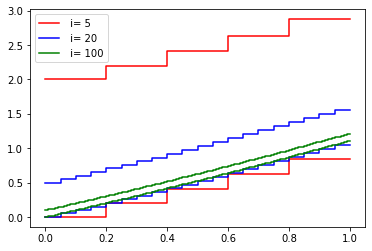
\includegraphics[scale=0.5]{./Figures/valit.png}
\caption{Cost functions for min and max adversaries at different partition granularities\label{fig:1dcosts}}
\end{figure}

\section{Q-learning}

In most cases the MDP $\mdp_{\partition,\alpha}$ will not be solvable analytically. Even for quite simple
examples of IMDPs and adversaries the transition probabilities $\alpha_T(\nu,a)$ are intractable.
However, if we can simulate the underlying EMDP, we can learn cost functions
and optimal strategies from observed runs. We here use Q-learning that for a given MDP $\mdp_{\partition,\alpha}$
aims to learn for each region-action pair $(\nu,a)$ the expected cost of performing action $a$ in
state $\nu$, and following an optimal strategy thereafter. The $Q$-values thus defined are initialized
as  $Q_0(\nu,a)=0$ for all $\nu,a$. Based on an observed run $\pi=\nu_0a_0\nu_1a_1\ldots\nu_ta_t\nu_{t+1}\ldots$
the $Q$-values are iteratively updated as
\begin{equation}
\label{eq:qlearn}
Q_{t+1}(\nu_t,a_t) = (1-\beta_t)Q_t(\nu_t,a_t) + \beta_t( \cost(\nu_t,a_t) + \lambda \min_{a\in\act}Q_t(\nu_{t+1},a)  ), 
\end{equation}
where $\beta_t\in(0,1)$ is the \emph{learning rate} at iteration $t$.
In order to ensure convergence with high probability,
$\beta_t$ is defined as a  decreasing function in the number of times the pair $(\nu_t,a_t)$ has been
updated at previous time points $s<t$\cite{jaakkola1993convergence}.
Thus, $\beta_t$ is a function of $\run_{0:t}$. Moreover, during
learning, actions $a_t$ are typically not selected according to a fixed, stationary strategy, but
according to a strategy that also is designed to collect data from previously under-explored
actions. This means that
actions are selected according to a histoy-dependent strategy
$
a_t=\sigma_t(\pi_{0:t}).
$
We write $\boldsigma=(\sigma_t)_t$ for such a history dependent strategy.
The data may also consist of multiple runs starting at the same or at different
initial state. For notational simplicity we take the data to consist of a single long sequence
indexed by $t$. 


Our goal is to approximate the true cost function $\expected(\cost_\lambda,s)$. In view of
(\ref{eq:alphabounds2}) it would be desirable to learn $\expected_{\alphamin}$ and
$\expected_{\alphamax}$ as strict lower and upper bounds from simulation runs of
$\mdp_{\partition,\alphamin}$ and $\mdp_{\partition,\alphamax}$, and to calibrate the diameter of
$\partition$ such that these bounds are sufficiently close. However, not only are the transition
probabilities defined by $\alphamin$ and
$\alphamax$ intractable to compute, but, since $\alphamin,\alphamax$ are only implicitly defined via
(\ref{eq:alphamin}) and  (\ref{eq:alphamax}), we often lack explicit representations of these adversaries that
could be used in simulations. We therefore use more tractable adversaries that can be
used efficiently in simulations.

The following definition defines adversaries in the form of random state selections. 


\begin{definition}
For each $(\nu,a)\in\partition\times\act$ let $\rho_{\nu,a}$ be a probability distribution on $\nu$.
The $\rho\emph{-adversary}$ $\alpharho$ is defined by
\begin{equation}
\label{eq:rhoadv}
\begin{array}{l}
\alpharho_T(\nu,a)(\nu'):=\int_\nu T(s,a,\nu')d\rho_{\nu,a}(s) \\
\alpharho_C(\nu,a):=\int_\nu \cost(s,a)d\rho_{\nu,a}(s)
\end{array}
\end{equation}
\end{definition}

The class of $\rho$-adversaries does not narrow down the class of adversaries significantly:
almost every adversary in the sense of
Definition~\ref{def:adversary}  is actually a $\rho$-adversary, with the possible exception
of adversaries that
pick $(\alpha_T(\nu,a),\alpha_C(\nu,a))$ on the boundary of  $T\cost^*_\partition(\nu,a)$.
However, the representation in form of a distribution $\rho$ allows us to characterized critical
computational properties of adversaries in the form of the following hierarchy of properties:

\begin{description}
\item[P1] For all $\nu,a$, one can  sample states $s\in\nu$ according to $\rho_{\nu,a}$
\item[P2] In addition to {\bf P1}, the cost values $\alpharho_C(\nu,a)$ can be computed for all $\nu,a$
\item[P3] In addition to {\bf P2}, the transition probabilities $\alpharho_T(\nu,a)(\nu')$ can be computed for all
$\nu,a,\nu'$. 
\end{description}

In all cases we assume that in the underlying EMDP we can sample successor states $s'$ according to
the distribution $T(s,a,\cdot)$, and that we can compute the cost $\cost(s,a)$. This means that
whenever $\rho$ is given by pointmass ${\boldsymbol 1}_s$ for some $s\in\nu$, and the mapping
$\nu\mapsto s\in\nu$ is explicitly given, then $\alpharho$ satisfies at least {\bf P2}.
This was the case in Example~\ref{ex:valit} for the min and max adversaries, where furthermore also
{\bf P3} was true. When {\bf P3} holds, then the resulting MDP can, in principle,
be solved by value iteration.

{\bf P2} is important because it is sufficient to support $Q$-learning: we can sample runs according to
the distribution
defined by $\mdp_{\boldsigma,\alpharho}$ for any (possibly non-stationary) strategy $\boldsigma$:
given a current state-action pair $(\nu,a)$, we sample a successor state $\nu'$ by randomly sampling
$s\in\nu$ according to $\rho$, then sampling $s'\in\states$ according to $T(s,a,\cdot)$, and finally
setting $\nu':=[s']_\partition$. If, according to {\bf P2}, we can at each step also compute the cost
value $\alpharho_C(\nu,a)$, then we obtain exactly the data needed for $Q$-learning. 


In many cases the implicit definition of  $\alphamin$ or $\alphamax$ will not allow for
their explicit  representation as an $\alpharho$, so that even  {\bf P1} does not hold.
We therefore consider the following more tractable explicit adversaries:
\begin{itemize}
\item $\rho_{\nu,a}$ is the uniform distribution on $\nu$, i.e., the Lebesgue measure normalized to a probability
distribution. Thus, $\rho_{\nu,a}$ does not depend on $a$. We then denote $\alpharho$ as $\alphamean$, and refer to
it as the \emph{mean-adversary}.
\item $\rho_{\nu,a}$ is the point mass that puts probability 1 on some state $s^{\emph{i-min}}\in\nu$ that has minimal
cost  $\cost(s,a)$ among all states of $\nu$.   We then denote $\alpharho$ as $\alphaimin$, and refer to
it as the \emph{immediate min-adversary}. $\alphaimin$ is a heuristic approximations of  $\alphamin$ that
is based on considering the immediate cost of the next transition only.
\item In analogy to $\alphaimin$, the \emph{immediate max-adversary} $\alphaimax$ is defined.
\end{itemize}


\begin{figure}
\centering
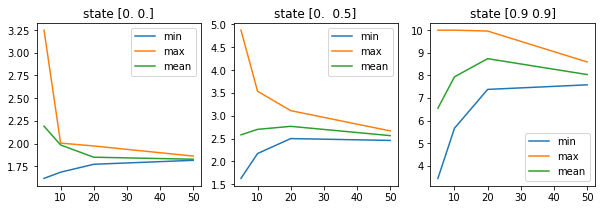
\includegraphics[scale=0.5]{./Figures/minmaxmean2d.png}
\caption{Cost values (y-axis) at selected states learned from partitions of granularities 5,10,20,50, (x-axis)
and the $\alphaimin, \alphaimax, \alphamean$ adversaries\label{fig:minmax2d}}
\end{figure}

\begin{example}
\label{ex:2dex-3}
(Example \ref{ex:2dex-2} continued). 
Similar to Example~\ref{ex:counterex} we consider partitions $\partition_i$ in the form of uniform grids with
region dimensions $1/i \times 1/i$.
For any region $\nu$ and all $a\in\act$ it is then easy to identify the
states $s\in\nu$ that minimize or maximize the cost $\cost(s,a)$, so that $\alphaimin$ and $\alphaimax$ are
given by explicit mappings $\nu\mapsto s\in\nu$, and  {\bf P2} holds. However, {\bf P3} does not hold for
$\alphaimin, \alphaimax$ as the integrals defining $\alphaimin_T,\alphaimax_T$ are over the cumulative
distribution function of the Gaussian distribution, for which no closed-form expression exists.
Thus, this model with  $\alphaimin_T,\alphaimax_T$ adversaries is amenable to $Q$-learning, but not
to analytic solutions. 

Considering the $\alphamean$ adversary, we find that this, too, satisfies {\bf P2}: clearly we can sample
states uniformly in a grid cell $\nu$. Also, due to the simple polynomial cost function (\ref{eq:2dcosts}), the
integrals defining $\alphamean_C(\nu,a)$ can be easily computed. 
Figure~\ref{fig:minmax2d} shows for three selected states in $\states$ the learned cost values
for $\cost_{0.6}$, of the regions
$[s]_{\partition_i}$ for $i=5,10,20,50$ under the $\alphaimin, \alphaimax, \alphamean$ adversaries.
For learning, we use a strategy $\boldsigma$ that always selects the next action uniformly at random, and
where the learning rate $\beta_t$ is $1/\sqrt{n}$, with $n$ the number of times $(\nu_t,a_t)$ has already
been updated.

Note that
according Theorem~\ref{prop:narrowbounds} all  costfunctions converge to
the true cost $\expected(\costlambda,s)$ as $i\rightarrow\infty$.
However, since $\alphaimin, \alphaimax$ only are approximations to the true min and max
adversaries, there is no strict guarantee that the $\alphaimin$ and $\alphaimax$ costs always provide
a lower and an upper bound on the actual cost. Still, as expected, the cost function for
$\alphamean$ lies in between $\alphaimin$ and $\alphaimax$, and provides better approximations to the
limit for the coarser partitions $\partition_i$. 

Figure~\ref{fig:succstates} on the right shows the strategy learned for $\mdp_{\partition_{50},\alphaimin}$
(the strategies learned for the $\alphaimax$ and $\alphamean$ adversaries look very similar). According
to the learned strategies one should try 
 to move to the middle of the state space, except when the current position is very close
 to the boundary, in which case it is preferable to perform the very cheap (but otherwise pointless) actions
 of moving into the boundary. 
\end{example}

% \begin{figure}
% 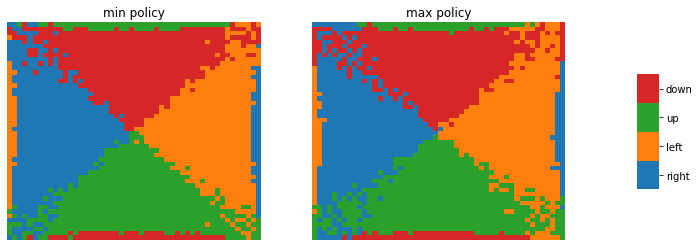
\includegraphics[scale=0.5]{./Figures/minmaxpolicy.png}
% \caption{Strategies learned under training with $\alphaimin$ and $\alphaimax$ adversaries \label{fig:minmaxadvs}}
% \end{figure}

While satisfied in the preceding example, even {\bf P2} can easily be out of reach. We now consider
an approach to approximating $Q$-learning for $\mdp_{\partition,\alpharho}$ when only {\bf P1} is true.
For any adversary $\alpharho$ with {\bf P1}, we can approximate simulations of
$\mdp_{\partition,\alpha^\rho}$ in a $Q$-learning scenario with a
non-stationary strategy $\boldsigma$ as follows:

\begin{itemize}
\item Given the current history $\pi_{0:t}$ and selected action $a_t=\sigma_t(\pi_{0:t})$:
\begin{itemize}
\item sample a state $s\in\nu_t$ according to $\rho_{\nu_t,a_t}$
\item return the cost value $\cost_t=\cost(s,a_t)$, and sample the next state $\nu'$ according to
$T(s,a,\nu')_{\nu'\in\partition}$.
\end{itemize}
\end{itemize}

This simulation generates runs $\nu_0a_0\nu_1a_1\ldots$ according to the distribution
$P_{\nu_0,\boldsigma}$ defined by  $\mdp_{\partition,\alpha^\rho}$, $\boldsigma$, and initial state $\nu_0$.
The simulations differ from exact simulations of $\mdp_{\partition,\alpha^\rho}$ (or any
MDP) in that the observed cost $\cost_t$ at step $t$ no longer is a function of the state-action pair
$(\nu_t,a_t)$.  However, one can still perform the Q-learning updates (\ref{eq:qlearn}) with
$\cost_t$ instead of $\cost(\nu_t,a_t)$. We denote the function defined by these updates at time
$t$ as $\tilde{Q}_t$. We now show that in expectation, we obtain the same results as with
standard $Q$-learning from proper simulations of  $\mdp_{\partition,\alpha^\rho}$.


\begin{theorem}
For all $(\nu,a)\in \partition\times\act$, $\nu_0\in\partition$, strategies $\boldsigma$, and $t\geq 0$:
\begin{equation}
\label{eq:expectations}
\expected_{\nu_0,\boldsigma}(\tilde{Q}_t(\nu,a))=\expected_{\nu_0,\boldsigma}({Q}_t(\nu,a))
\end{equation}
\end{theorem}


\begin{proof}
By induction on $t$. For $t=0$ we have $\tilde{Q}_0\equiv Q_0 \equiv 0$. Assume (\ref{eq:expectations})
holds for $t$. Then we first write
\begin{equation}
\expected_{\nu_0,\sigma}(\tilde{Q}_{t+1}(\nu,a)) =
\sum_{\path_{0:t}\in \partition^t} P_{\nu_0,\boldsigma}(\path_{0:t})\expected_{\nu_0,\sigma}(\tilde{Q}_{t+1}(\nu,a)|\path_{0:t}),
\end{equation}
and similarly for $\expected_{\nu_0,\sigma}({Q}_{t+1}(\nu,a))$. Since the probabilities
$P_{\nu_0,\boldsigma}(\path_{0:t})$ are the same for $\tilde{Q}_{t}$ and ${Q}_{t}$, it is sufficient to show
that for all $\path_{0:t}$
\begin{equation}
\expected_{\nu_0,\sigma}(\tilde{Q}_{t+1}(\nu,a)|\path_{0:t})=\expected_{\nu_0,\sigma}({Q}_{t+1}(\nu,a)|\path_{0:t}).
\end{equation}
If $\nu_{t}\neq \nu$ in $\path_{0:t}$, or $a\neq \sigma_t(\path_{0:t})$, then the $Q$ and $\tilde{Q}$ values
of $(\nu,a)$ are not updated in the $t+1$'st iteration, and (\ref{eq:expectations}) holds by induction
hypothesis.

Assume, then, that $(\nu_{t}a_{t})=(\nu,a)$. We obtain:
\begin{multline}
\label{eq:local190}
\expected_{\nu_0,\boldsigma}(\tilde{Q}_{t+1}(\nu,a)|\path_{0:t})= 
(1-\beta_{t}(\path_{0:t}))\expected_{\nu_0,\boldsigma}(\tilde{Q}_{t}(\nu,a)|\path_{0:t}) +\\
\beta_{t}(\path_{0:t})(\expected_{\nu_0,\boldsigma}(\cost_{t}|\path_{0:t})+
\lambda \expected_{\nu_0,\boldsigma}(\min_{a'\in\act}\tilde{Q}_{t}(\nu_{t+1},a)|\path_{0:t}) ),
\end{multline}
where in the rightmost term the $\tilde{Q}_{t}(\nu_{t+1},a)$ now are to be understood as random
variables defined by the random next state $\nu_{t+1}$. 
The distribution of $\cost_t$ conditional on $\path_{0:t}$ only depends on $\nu_t=\nu$, and the expectation is
\begin{equation}
\label{eq:local200}
\expected_{\nu_0,\boldsigma}(\cost_{t}|\path_{0:t})=\int_\nu \cost(s,a) d\rho_{\nu,a}(s)=\alpha^\rho_C(\nu,a).
\end{equation}
The distribution for the random $\nu_{t+1}$ given $\path_{0:t}$
only depends on $\nu_t$ and $a=a_t=\sigma_t(\path_{0:t})$. We can therefore write: 
\begin{multline}
\label{eq:local210}
\expected_{\nu_0,\boldsigma}(\min_{a'\in\act}\tilde{Q}_{t}(\nu_{t+1},a)|\path_{0:t}) = 
\int_\nu  \sum_{\nu'\in\partition} T(s,a,\nu')  \min_{a'\in\act} \tilde{Q}_{t}(\nu',a') d\rho(s) =\\
\sum_{\nu'\in\partition} \min_{a'\in\act} \tilde{Q}_{t}(\nu',a') \int_\nu  T(s,a,\nu') d\rho(s) =
\sum_{\nu'\in\partition} \alpha^\rho_T(\nu,a)(\nu')   \min_{a'\in\act} \tilde{Q}_{t}(\nu',a').
\end{multline}
Substituting the right-hand sides of (\ref{eq:local200}) and (\ref{eq:local200}) into the
right-hand side of (\ref{eq:local190}), and replacing by induction hypothesis
$\tilde{Q}_t$ with $Q_t$ everywhere, we obtain
\begin{multline}
(1-\beta_{t}(\path_{0:t}))\expected_{\nu_0,\boldsigma}({Q}_{t}(\nu,a)|\path_{0:t}) +\\
\beta_{t}(\path_{0:t})(\alpha^\rho_C(\nu,a)  +
\lambda \sum_{\nu'\in\partition} \alpha^\rho_T(\nu,a)(\nu') \min_{a'\in\act}\tilde{Q}_{t}(\nu_{t+1},a) =\\
\expected_{\nu_0,\sigma}({Q}_{t+1}(\nu,a)|\path_{0:t}).
\end{multline}

\end{proof}

\begin{figure}
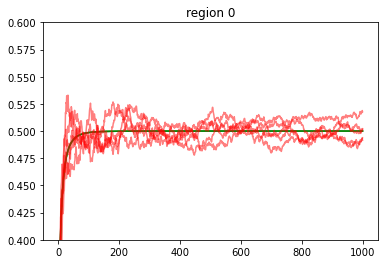
\includegraphics[scale=0.5]{./Figures/region0.png}
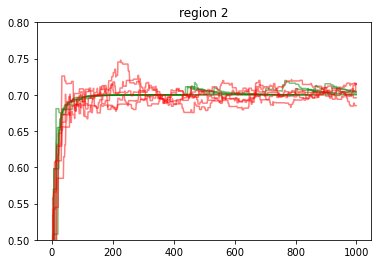
\includegraphics[scale=0.5]{./Figures/region2.png}
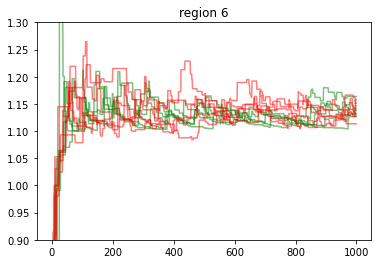
\includegraphics[scale=0.5]{./Figures/region6.png}
\caption{Learned $Q$ vs. $\tilde{Q}$-values for selected regions \label{fig:Qcurves}}
\end{figure}

\begin{example}
\label{ex:2dex-4}
(Example \ref{ex:2dex-3} continued).
We consider the $\alphamean$ adversary, and compare the $Q$-values learned during proper $Q$-learning with
the $\tilde{Q}$ values obtained during our approximation of the $Q$ learning process. 

For both exact and approximate $Q$-learning we perform 5 learning
runs. In each learning run we sample 1000 times a random initial state, and then simulate
system runs of length 10 (since in this model runs quickly get absorbed in the leftmost
region, many short runs are needed to collect informative data). We record the $Q$ and $\tilde{Q}$ values
at the end of each short run. 

Figure~\ref{fig:Qcurves} shows for regions $[0,0.1[,[0.2,0.3[$ and $[0.6,0.7[$ the developments of the
$Q$ (green) and $\tilde{Q}$ (red) values over the course of the 1000 episodes. One can see that in expectation
the learned $Q$ and $\tilde{Q}$ coincide, but that the  $\tilde{Q}$ values exhibit a larger variance. For the
region $[0.6,0.7[$ further to the right also the $Q$-values show significant variance. This is because
the values here are supported by much fewer datapoints.
\end{example}



\section{Bouncing ball}

\section{Conclusion}

Open problem: interleaving with refinement steps

\bibliographystyle{abbrvnat}
\bibliography{imdp}

%\input{appendix}
\end{document}
